\section{Waveform analysis}
\label{sec:Analysis}


A fast data analysis was performed within hours or days from the data
acquisition. Each waveform is analysed individually, through a few
steps:

\begin{itemize}
\tightlist
\item
  baseline identification: average of the central 50\% of the samples
\item
  RMS: RMS of the samples used in the baseline determination
\item
  extrema determination: amplitude of the positive and negative peaks
  along the whole waveform
\end{itemize}


For each channel, the parameters from all the available waveforms (10)
are averaged to extract:

\begin{itemize}
\tightlist
\item
  baseline RMS (RMS of the 10 baselines)
\item
  noise average (average of the 10 RMS, one for of each baseline)
\item
  peak amplitude average and its uncertainty (the positive
  peak from each waveform are averaged)
\end{itemize}

This analysis is aimed for speed, and it can definitely be refined.

% ----------------------------------------------------------------------
\subsection{Baseline and RMS identification}
\label{sec:baseline-and-rms-identification}


The principle is to exclude the signal, intended as the response to the
pulse, and to use the remaining of the waveform to estimate the
baseline. The algorithm is designed not to require prior knowledge of
the position or shape of the peaks.\\

The signal is shaped as two sharp-rising peaks, which including the
decay tails are roughly 200 µs or shorter. The algorithm relies on the
assumption that those two peaks are indeed roughly that narrow, although
it does not assume anything on their size or shape. It flows as follows:

\begin{enumerate}
\tightlist
\item
  sort all the 10000 samples in increasing order; in this way, the
  samples taken during the negative peak will be at the left of the
  data, the ones at the positive peak will be at its right, and the
  middle of the data will be populated by long sequences of samples with
  similar values, from the baseline
\item
  select the samples from \#2500 to \#7499 from the sorted data for
  further analysis
\item
  take the average and RMS of the selected samples, which will represent
  the baseline and noise respectively
\end{enumerate}

This algorithm may present some bias if the tail from the first peak
overlaps the second peak. An alternative, simple algorithm would rely on
the assumption that the peak is on the second half of the waveform, and
would therefore use the first 40\% or 50\% of the waveform for baseline
determination as in the last point of the algorithm.\\

An older version of the algorithm would rely of the knowledge of the
peak position, and would fail when the waveform does not contain any
actual signal.


% ----------------------------------------------------------------------
\subsection{Peak determination}
\label{sec:peak-determination}


Again a simple algorithm, the peak determination consists of two simple
steps:

\begin{enumerate}
\tightlist
\item
  determine the absolute maximum and minimum of the waveform
\item
  subtract to both the baseline (obtained separately)
\end{enumerate}

This algorithm is affected by the noise on the waveform, which can be
quantified together with the baseline. Although this is less than ideal,
the actual noise has been measured to be low enough to be not
significant for the purpose of the fast analysis we performed{[}1{]}.\\

{[}1{]} In more recent versions of the library, the minimum and maximum
are not evaluated from the single sample, but replaced by a running
window average on 5 samples.


% ----------------------------------------------------------------------
\subsection{Results}
\label{sec:results}

We summarize the results of the baseline, RMS, positive peak value, 
and the ratio of the positive peak value to the baseline in 
\Cref{fig:baseline,fig:rms,fig:pospeak,fig:pospeaktobaseline}.
Each strip represents a single channel of the detector.
The x-axis includes all the chimneys of the ICARUS detector, while
the y-axis shows all the 18 cables, each with 32 channels, within a chimney.
The color code in each figure indicates the values of the baseline, the RMS,
the positive peak, or the ratio of the positive peak value to
the baseline value.\\

The corner chimneys, Ch01 and Ch20 in each row, have only the channels
connecting to horizontal wires, where the data was not recorded in this
round of the connectivity test and therefore is not shown in the plots.
Cables 1-9 in Ch02 and Ch03 and cables 10-18 in Ch18 and Ch19 are connected
to the corner wires in the second induction and collection planes which are
shorter in length.
Owing to their ending points, the cables injecting the test pulse are
not located at the same chimney.
Without the information of the location of the pulse-injecting cables,
we are not able to obtain a result of these wires, and 
\Cref{fig:pospeak,fig:pospeaktobaseline} show extremely low or
overflown values.\\


% ----------------------------------------------------------------------
\begin{figure}
\centering
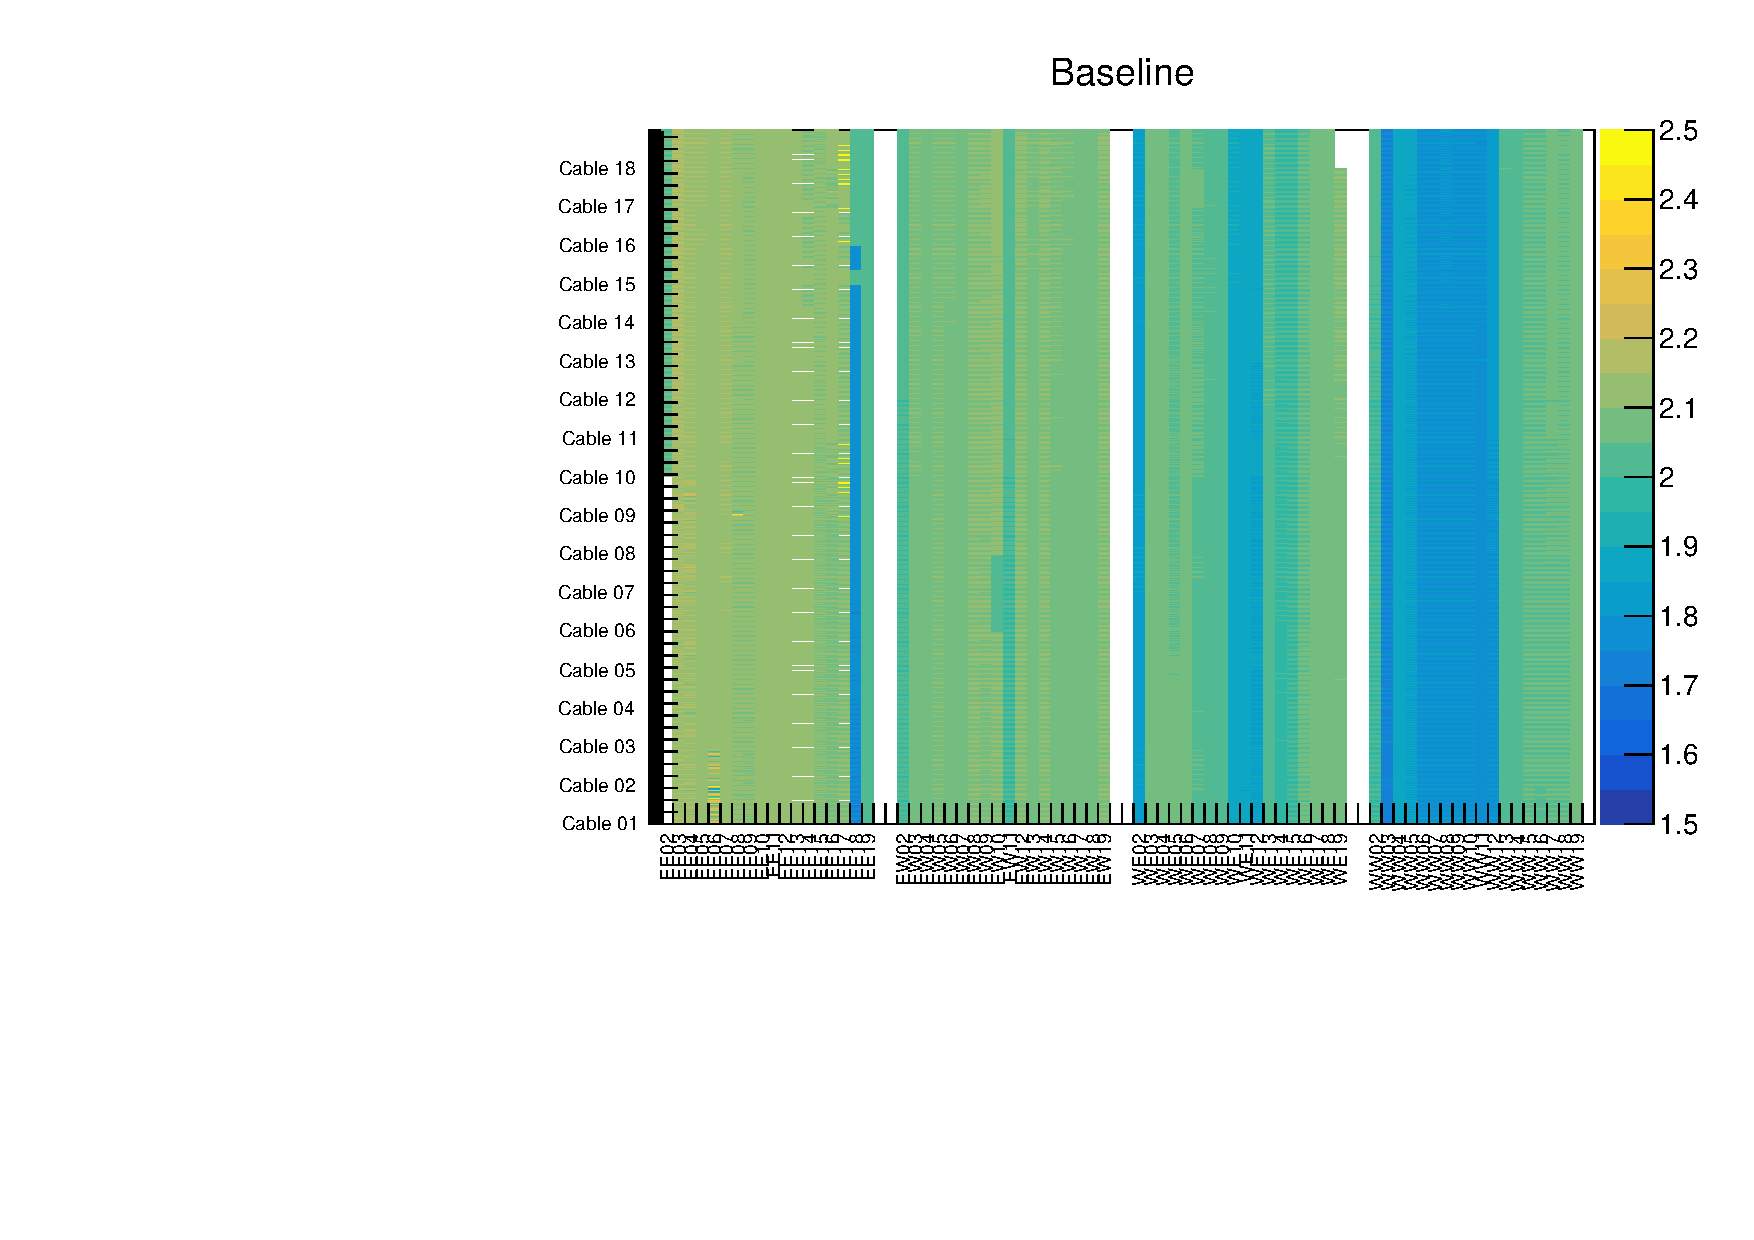
\includegraphics[width=\textwidth]{fig/Baseline.pdf}
\caption{The map of the baseline values of all the channels.
Each strip represents a single channel of the detector.
The x-axis includes all the chimneys of the ICARUS detector, while
the y-axis shows all the 18 cables, each with 32 channels, within a chimney.
The color code in each figure indicates the values of the baseline.}
\label{fig:baseline}
\end{figure}
% ----------------------------------------------------------------------

% ----------------------------------------------------------------------
\begin{figure}
\centering
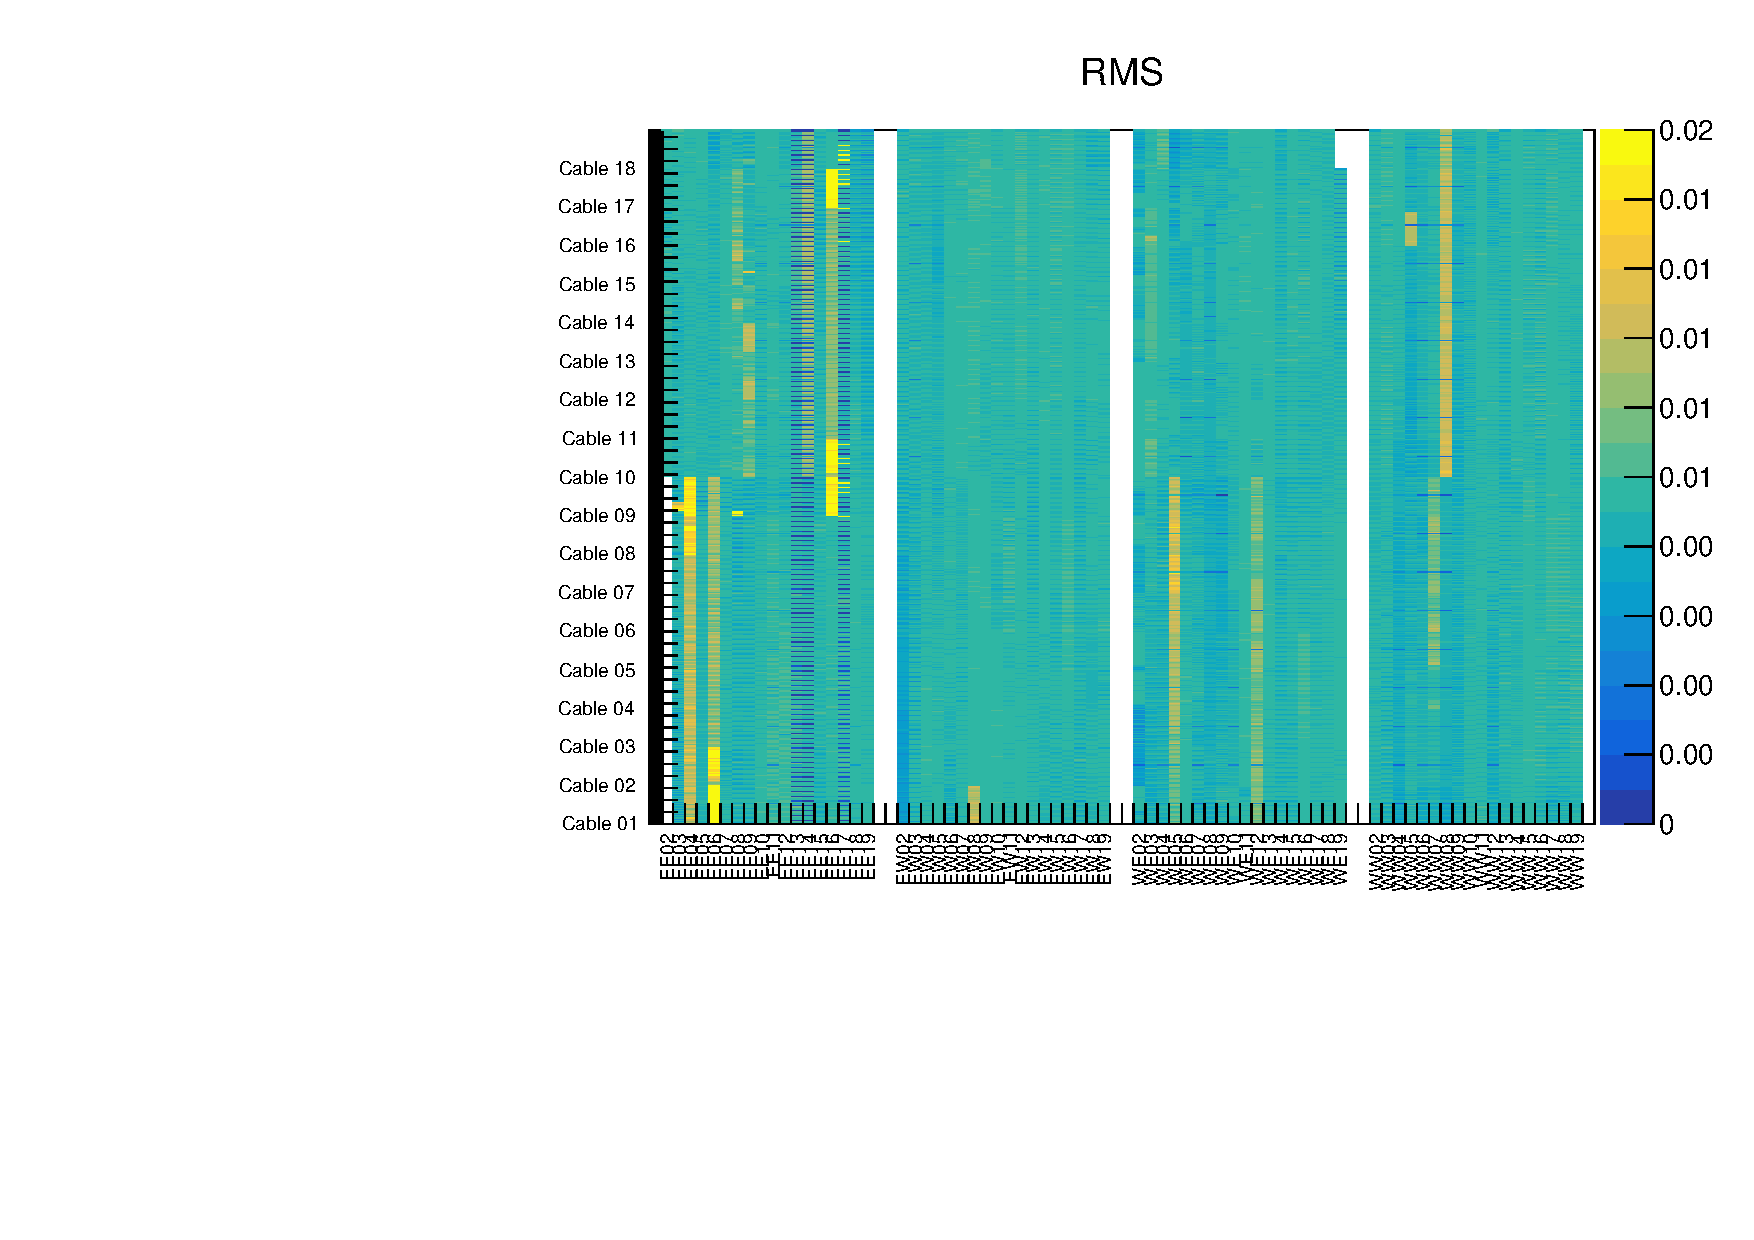
\includegraphics[width=\textwidth]{fig/RMS.pdf}
\caption{The map of the RMS of all the channels.
Each strip represents a single channel of the detector.
The x-axis includes all the chimneys of the ICARUS detector, while
the y-axis shows all the 18 cables, each with 32 channels, within a chimney.
The color code in each figure indicates the values of the RMS.}
\label{fig:rms}
\end{figure}
% ----------------------------------------------------------------------

% scale in the oscilloscope
In chimneys EE13, EE14, and EE17, the white strips in \Cref{fig:baseline} 
and the dark blue strips in \Cref{fig:rms,fig:pospeak},
indicating extremely low values,
appear in every four channels.
It is owing to the fact that the fourth channel in the oscilloscope
happens to be set a larger scale in voltage, and, as a consequence, 
the relative values of the baseline and the pulse peak are small.
The effect is canceled out in \Cref{fig:pospeaktobaseline}, where the
ratio of the peak to baseline values is plotted.\\

% dead channel in the test box
The fifth channel of the connector for the flat ribbon cables in a test
box is damaged, and we are not able to read out the signals from the
channel when using this test box.
It thereby shows the dark blue strips in chimneys EE10-14, EW 03-07,
WE02-12, and WW03-12 in \Cref{fig:pospeak,fig:pospeaktobaseline}.
Nonetheless, this round of the connectivity test aims to identify
potential problems in terms of cables, and a single damaged channel
in the test box should not affect the effectivity.\\

% voltage
Since there is no voltage regulator for the battery powering the test
boxes, the baseline value, which is set to the half of the voltage,
decreases as the time being, as shown in \Cref{fig:baseline}.
Hence, \Cref{fig:pospeaktobaseline}, which cancels out the baseline
decrease, gives us a more uniform comparison across the whole detector.\\

% special cables
In the EE and WE rows, cables 1-8, cable 9, cables 10-17, and cable 18
have separate pulse-injecting cables, while in the EW and WW rows, those
groups are cable 1, cables 2-10, cable 11, and cables 12-18.
During the tests, we do not have the information on this grouping of
wires, except that cables 1-9 and 10-18 are for induction and collection
wires, respectively, and have different pulse-injecting cables.
Consequently, for some chimneys, cables 1-9 are tested with
the same pulse-injecting cable, and so are cables 10-18; 
for other chimneys, cables 1-8, 10, 11-17, and 18 are tested with different
pulse-injecting cables.
With the cross talk effect discussed in the next paragraph,
it is not straightforward to distinguish whether the measured signal
corresponds to the injected pulse or the cross talk signal in the special
cables, cables 9 and 18 in the EE and WE chimneys and cables 1 and 11
in the EW and WW chimneys.
In addition, it is raised that the grouping of the channels for the same
pulse-injection cables might be cables 1-8, 9, 10-17, 18 for the chimney
EE02, but cables 1, 2-10, 10-17, 18 for the next chimney, EE03, and
similar patterns for other chimneys.
However, we have not reached a conclusive statement by analyzing the
current data, which convolved several issues including the cross talk,
potentially wrong cables for pulse-injection, etc.
We defer the conclusion to the next iteration of connectivity test
where we expect to have equipment disentangling those issues.\\

% cross talk
The wires involved in the connectivity test should normally not be connected
to the detector ground, but it was observed that some of them are during the
overhaul at CERN.
The design of the test box in this iteration does not connect the wire cables
to the detector ground, and therefore in the normal case of the wire grounding,
the cross talk from the adjacent twisted wires contributes a significant
portion to the signal.
Roughly speaking, the amplitude of the cross talk signal is similar to
to that of the injected pulse, which severely complicates the signal
interpretation.
In the normal case, where the wire is correctly connected but not grounded 
to the detector, the signal will be the superposition of the injected
pulse and the cross talk signal.
On the other hand, in the cases that the wire is not connected and not
grounded, and that the wire is connected and also grounded,
the signal will contain, respectively, only the cross talk and only the
injected pulse, both of which will have roughly half the amplitude of
the signal in the normal condition.
By analyzing all the possible scenarios listed in \Cref{table:crosstalk},
we ensure the connectivity of the channels with the full size amplitude in
\Cref{fig:pospeaktobaseline}.
Further, to distinguish the connected wires among those with the half 
size amplitude, such as cable 8 in chimney WW06, cables 4 and 17 in chimney WW12,
we explicitly check their grounding.
The check confirms those wires are grounded and we are reading the injected
pulse but not the cross talk from adjacent wires.\\

\begin{table}
\centering
\begin{tabular}{ccc}
\hline
\hline
    & Shield grounded  & Shield isolated \\
\hline
Cable connected & 1/2 size signal & Full size signal \\
Cable disconnected & No signal & 1/2 size signal \\
\hline
\hline
\end{tabular}
\caption{The qualitative signal amplitudes of all the
possible scenarios of shield grounding and
wire connection.}
\label{table:crosstalk}
\end{table}


% ----------------------------------------------------------------------
\begin{figure}
\centering
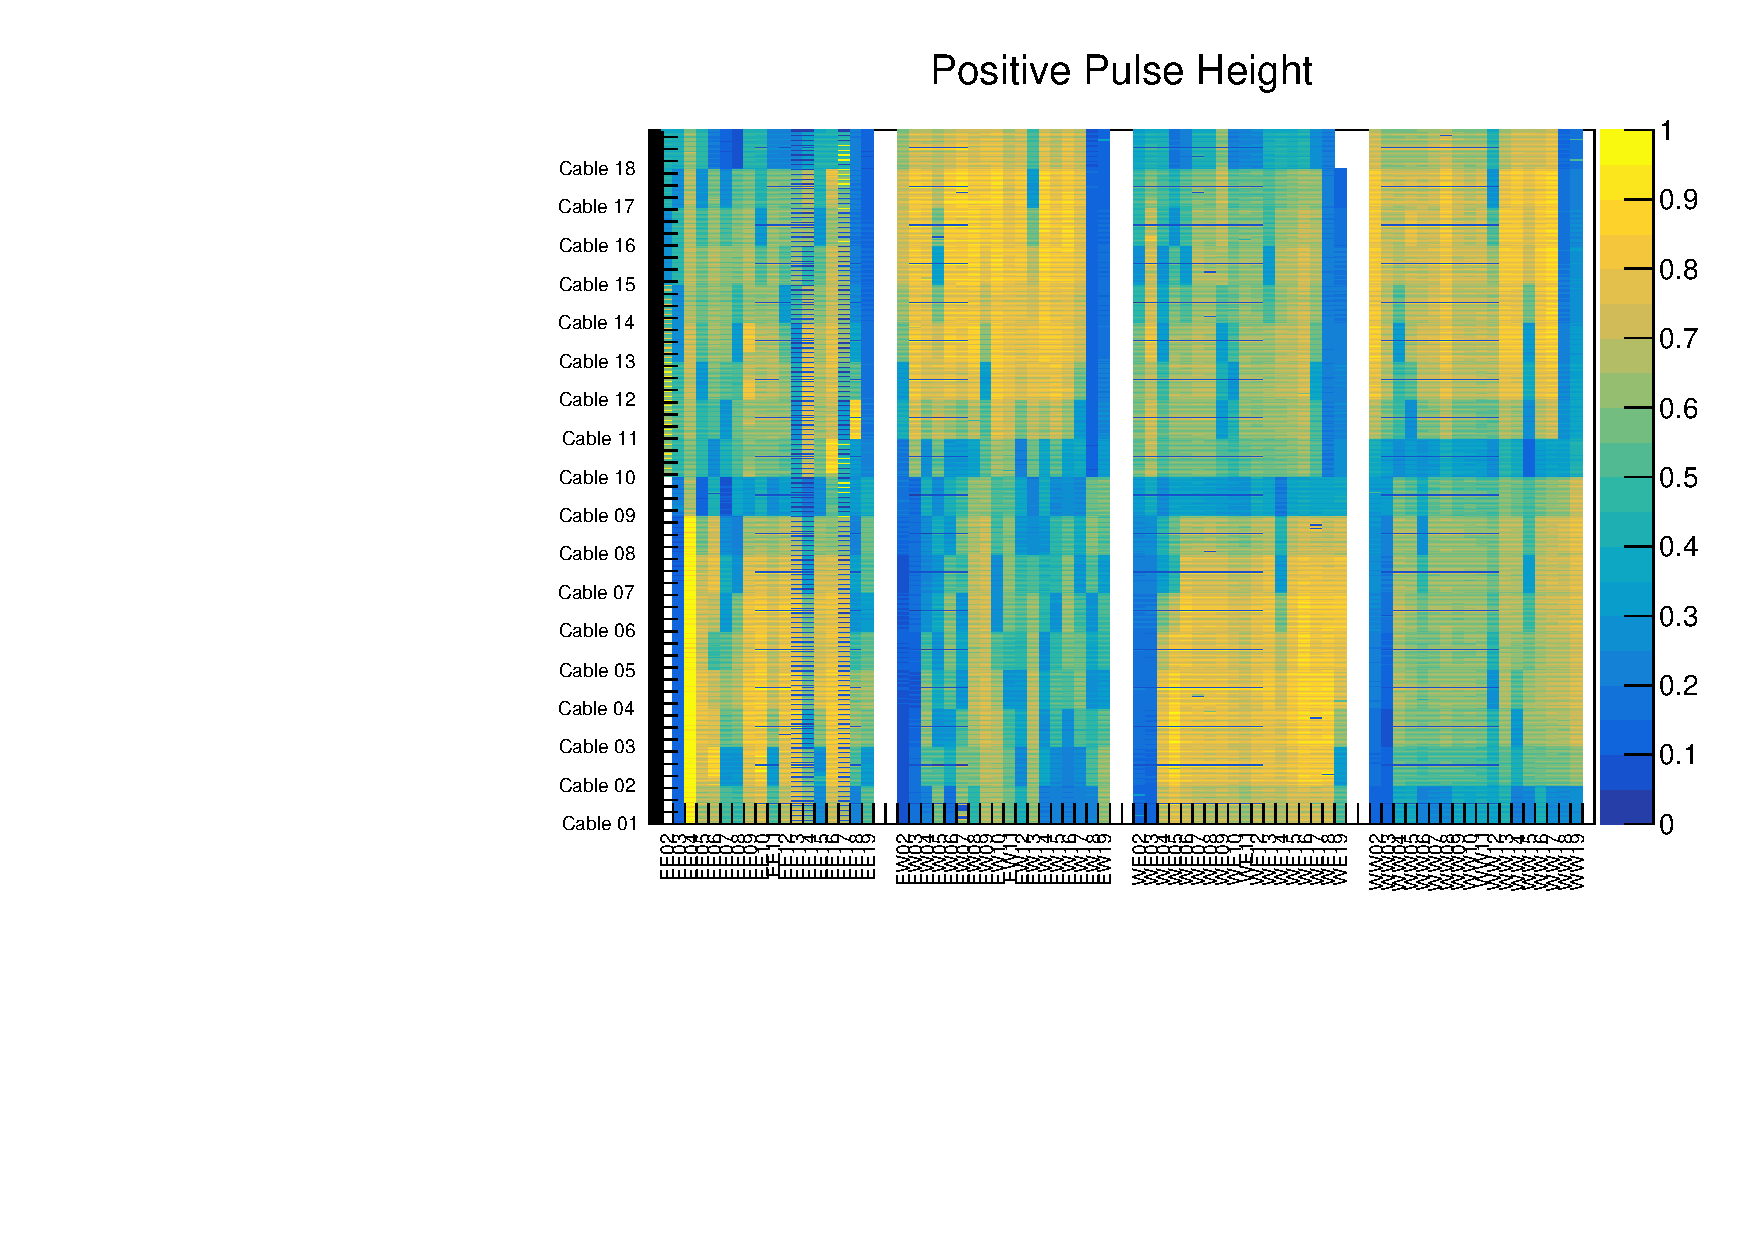
\includegraphics[width=\textwidth]{fig/PosPeak.pdf}
\caption{The map of the positive peak values of all the channels.
Each strip represents a single channel of the detector.
The x-axis includes all the chimneys of the ICARUS detector, while
the y-axis shows all the 18 cables, each with 32 channels, within a chimney.
The color code in each figure indicates the values of the positive peak.}
\label{fig:pospeak}
\end{figure}
% ----------------------------------------------------------------------

% ----------------------------------------------------------------------
\begin{figure}
\centering
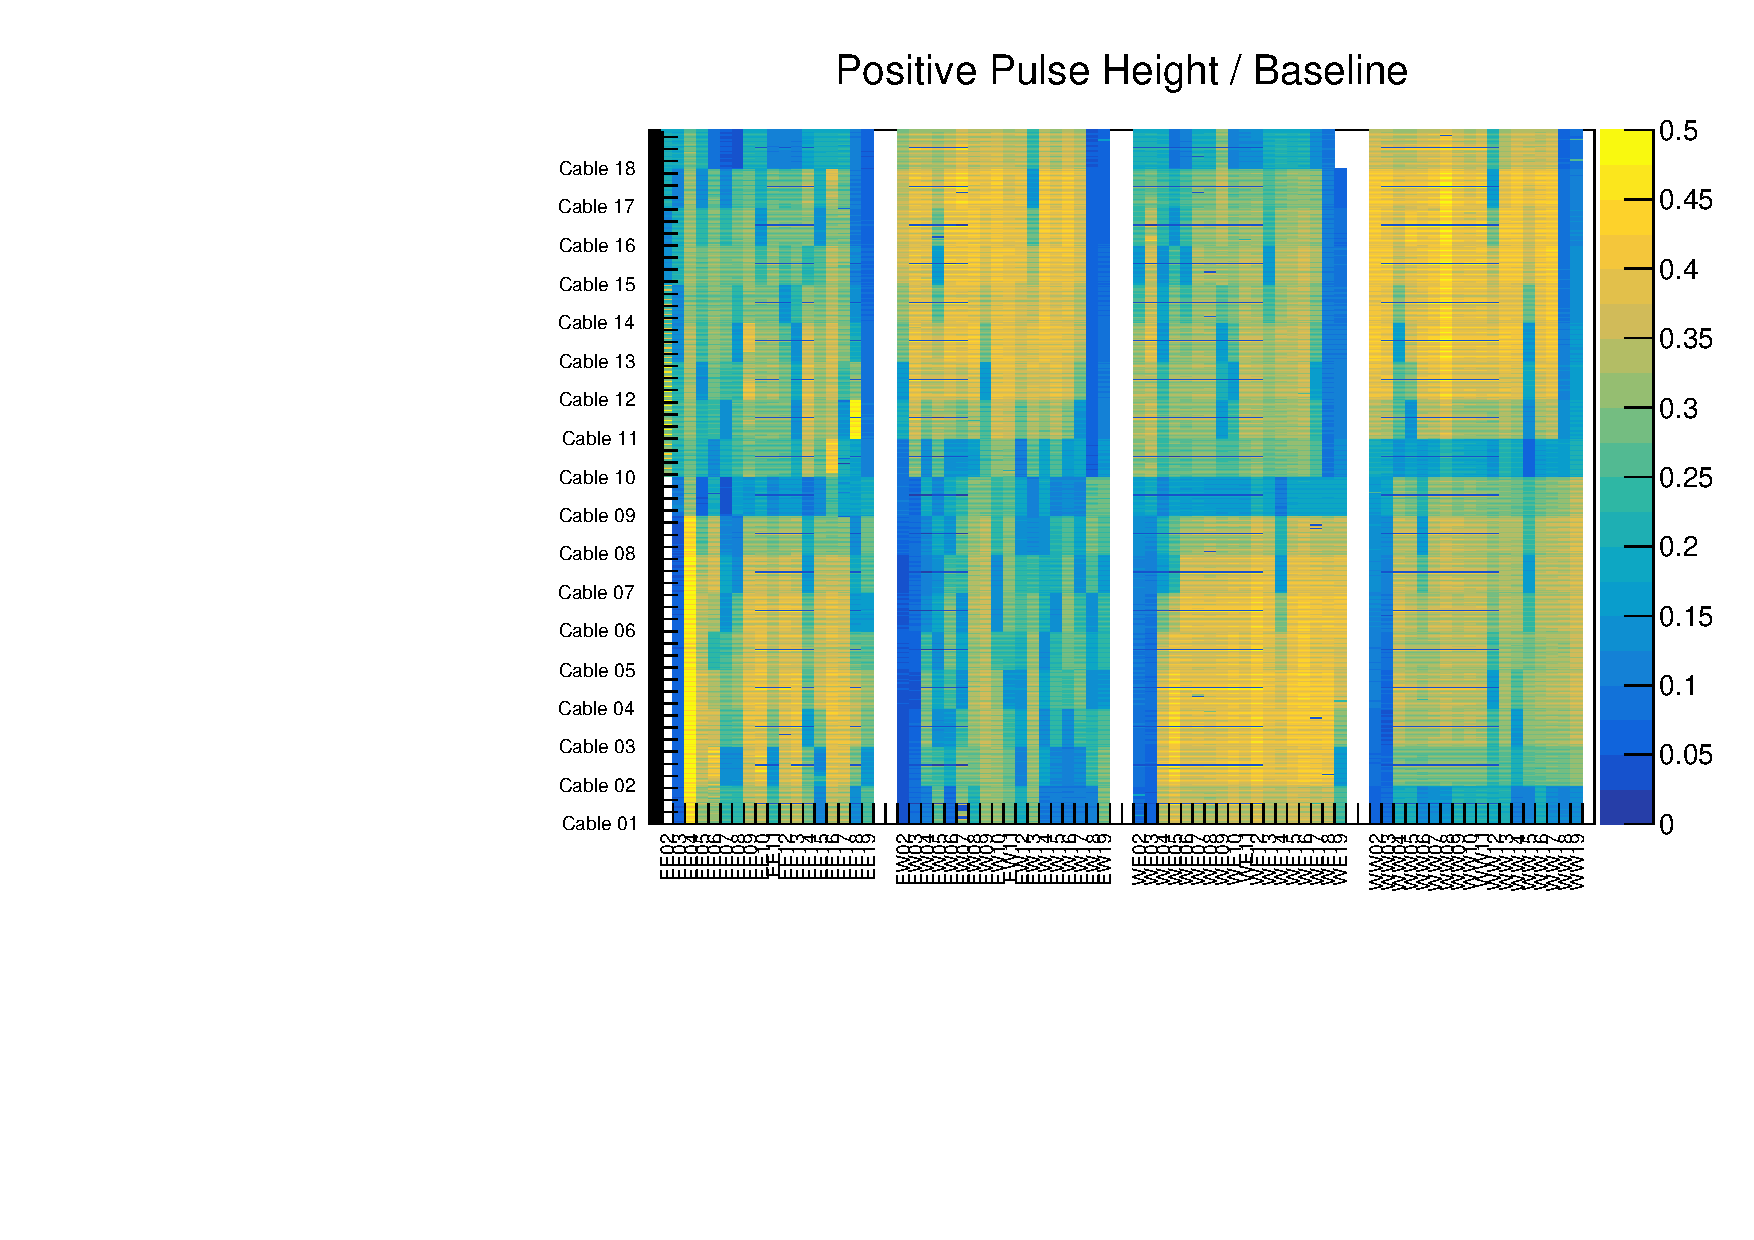
\includegraphics[width=\textwidth]{fig/PosPeakToBaseline.pdf}
\caption{The map of the positive peak to baseline ratios of all the channels.
Each strip represents a single channel of the detector.
The x-axis includes all the chimneys of the ICARUS detector, while
the y-axis shows all the 18 cables, each with 32 channels, within a chimney.
The color code in each figure indicates the values of the ratio.}
\label{fig:pospeaktobaseline}
\end{figure}
% ----------------------------------------------------------------------

% fine structure in the same cable
\Cref{fig:pospeaktobaseline} shows slight non-uniformity
in the signal amplitude of some cables, 
such as cables 10-13 in chimney EE09.
Looking into the values of those cables, we clarify those cables do not
have particularly non-uniform signal amplitudes, and the effect shown
in \Cref{fig:pospeaktobaseline} is rather owing to the color scale.\\

% conclusion
We conclude that there is no disconnected cable, and the source of all 
the cables with lower signal amplitude is confirmed to be the grounding.


